%!TEX root = ../EmbSW1.tex
\section{Concurrency}

\subsection{Motivation}
\subsubsection{Wieso wird Concurrency verwendet?}
\begin{itemize}
  \item Praktische Programme führen meist mehrere Arbeiten "`gleichzeitig"' aus.
\end{itemize}

\subsubsection{Parallel vs. Concurrent Computing}
\begin{itemize}
  \item Parallel Computing
  	\begin{itemize}
  	  \item execution of different tasks is really at the same time
  	  \item is not possible on a single-core machine
  	\end{itemize}
  \item Concurrent Computing
  	\begin{itemize}
  	  \item execution of different tasks only seems to be at the same time
  	  \item different tasks get consecutive time slices
  	  \item there's only one task really running at a particular time slice
  	  \item can be done on a single- or multicore machine
  	\end{itemize}
\end{itemize}

\subsubsection{Gründe, Concurrency nicht zu verwenden}
\begin{itemize}
  \item \textbf{Concurrency (mit Prozessen, Tasks, Threads) kostet immer}:
  \begin{itemize}
  	\item Stack
  	\item Context switch (Umschalten vom einen zum anderen)
  	  \begin{itemize}
  	  \item dauert
  	  \item Alter Context muss gespeichert, neuer wieder geladen werden
  	  \end{itemize}
  	\item Zugriff auf gemeinsame Ressourcen muss synchronisiert werden
  	  \begin{itemize}
  	  \item kostet
  	  \item fehleranfällig (wird vergessen oder falsch gemacht)
  	  \end{itemize}
  \end{itemize}
\item \textbf{Komplexität steigt}
  \begin{itemize}
  \item Sequentielle Programme sind einfacher zu verstehen als parallele
  \item Ziel ist immer, ein System möglichst einfach zu halten
  \end{itemize}
\end{itemize}

\textbf{Folgerung:} Concurrency nur dann einsetzen, wenn wirklich ein Nutzen vorhanden ist!\\
Tendenziell werden speziell bei Verwendung eines RTOS zu viele Threads definiert, welche das System nur komplexer und komplizierter machen $\rightarrow$ \textbf{Sequential} is simple, \textbf{concurrent} is error-prone

\subsection{POSIX Threads Programming}
\subsubsection{UNIX Process}
\begin{itemize}
  \item Heavyweight process (created by the operating system)
  \item Processes require a fair amount of overhead; they contain information about program resources and program execution state, including: Process ID, process group ID, user ID, and group ID; Environment; Program instructions; Registers; Stack; Heap; File descriptors; Signal actions; Shared libraries; Inter-process communication tools
\end{itemize}

\subsubsection{UNIX Thread}
\begin{itemize}
  \item Lightweight "'process"'
  \item \textbf{Threads use and exist within the process resources}
  \item \textbf{A thread uses the same address space as other threads of the same process}
  \item Threads are able to be scheduled by the operating system
  \item Independent stream of instructions that may run simultaneously to other streams of instructions
  \item Procedure that runs independently from its main program
  \item A thread maintains its own: Stack pointer; Registers; Scheduling properties; Set of pending and blocked signals; Thread specific data
  \item Concurrent programs are usually achieved with threads
\end{itemize}

\subsubsection{Process vs. Thread in UNIX}
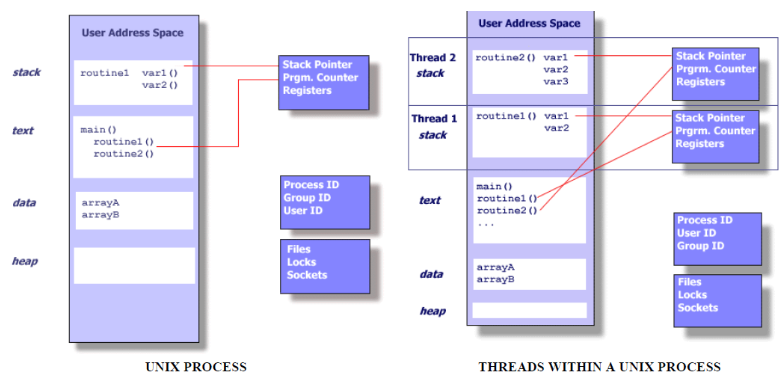
\includegraphics[width=12cm]{images/Concurrency/ProcessVsThread.png}\\\\
Man beachte: Alles was ein Thread inne hat, hat ein Prozess auch inne (aber NICHT umgekehrt)!

\subsection{What are POSIX Threads?}
\begin{itemize}
  \item For UNIX systems, a standardized C language threads programming interface has been specified by the \textbf{IEEE POSIX 1003.1c standard}.
  \item The short form of \textbf{POSIX threads} is \textbf{Pthreads} or \textbf{pthreads}.
  \item When compared to the cost of creating and managing a process, a thread can be created with much less operating system overhead
  \item Managing threads requires fewer system resources than managing processes
\end{itemize}

\subsubsection{The pthreads API}
\begin{itemize}
  \item Routines of the pthreads API start with \textbf{pthread\_}
  \item The header file \textbf{pthread.h} must be included
  \item Source files that use pthreads shall be compiled and linked with \textbf{-pthread}
  \item The link command must include \textbf{–lpthread}
\end{itemize}

\subsubsection{Starting and Terminating a Thread}
\begin{itemize}
  \item Any routine with the following interface may become a thread routine:\newline
  \lstinline{void* threadRoutine(void* arg);}
  \item A thread is started with:\newline
  \lstinline{int pthread_create(pthread_t* thread, const pthread_attr_t* attr, void* (*startRoutine) (void*), void* arg);}
  \begin{itemize}
  \item thread: pointer to a pthread\_t instance
  \item attr: pointer to a pthread\_attr\_t structure, often 0 (default attributes)
  \item arg: a single argument that may be passed to startRoutine
  \item returns 0 on success
  \end{itemize}
\item A thread terminates in one of the following ways:
  \begin{itemize}
  \item it calls pthread\_exit()
  \item it returns from startRoutine
  \item it is canceled with pthread\_cancel()
  \end{itemize}
\end{itemize}
\textbf{Example - Starting a Thread}
\begin{lstlisting}[style=C, escapechar=!]
#include <pthread.h>
void* threadFunction(void* arg);
int main(void)
{
  pthread_t myT; !\tikz[remember picture] \node [] (a) {};!
  int ret = pthread_create!\tikz[remember picture] \node [] (b) {};!(&myT, 0, threadFunction, 0);
  if (ret)
  {  // handle error
    return -1;
  }
  while (1) {} // endless loop
  return 0;
}
void* threadFunction(void* arg)
{  // implement this
  return 0;
}
\end{lstlisting}
\begin{tikzpicture}[remember picture, overlay,
  every edge/.append style = { ->, thick, >=stealth, dashed, line width = 1pt},
  every node/.append style = { align = left, minimum height = 10pt, font = \bfseries, fill= green!20},
  text width = 5.5cm]
  \node [right=8cm of a] (A) {myT becomes the reference to the thread};
  \node [below right=.5cm and 3cm of b, text width=8.5cm] (B) {starts thread and immediately returns (thread may not yet be fully started)};
  \draw (A.west) edge (a.east);
  \draw[->, to path={-| (\tikztotarget)}] (B.west) edge (b.south);
\end{tikzpicture}
\newpage
\textbf{Example - Waiting on a Thread to Finish}
\begin{lstlisting}[style=C, escapechar=!]
#include <pthread.h>
void* threadFunction(void* arg);
int main(void)
{
  pthread_t myT;
  int ret = pthread_create(&myT, 0, threadFunction, 0); // only starts and returns
  if (ret)
  {  // handle error
    return -1;
  }
  ret = pthread_join(myT, 0);!\tikz[remember picture] \node [] (a) {};!
  if (ret)
  {  // handle error
    return -1;
  }
  return 0;
}
void* threadFunction(void* arg)
{  // implement this
  return 0;
}
\end{lstlisting}
\begin{tikzpicture}[remember picture, overlay,
  every edge/.append style = { ->, thick, >=stealth, dashed, line width = 1pt},
  every node/.append style = { align = left, minimum height = 10pt, font = \bfseries, fill= green!20},
  text width = 7.5cm]
  \node [right=5cm of a] (A) {main thread waits on myT to finish};
  \draw (A.west) edge (a.east);
\end{tikzpicture}
%\lstinputlisting[style=C]{snippets/Threads/thread_waiting.c}

\subsubsection{Thread-safeness}
\begin{itemize}
  \item Thread-Sicherheit besagt, dass eine Komponente gleichzeitig von verschiedenen Programmbereichen mehrfach ausgeführt werden kann, ohne dass diese sich gegenseitig behindern.
  \item Änderungen der einzelnen Threads müssen koordiniert werden, um einen chaotischen Zustand des Speichers zu verhindern, da das Programm dabei häufig gleichzeitig auf einen gemeinsamen Speicherbereich (Shared Memory) des Computers zugreifen will.
  \item Vorsicht: rand() ist nicht thread-safe (weil bei dieser Fkt. eine interne Variable verwendet wird, welche schon zum Voraus berechnet wurde); rand\_r() hingegen schon.
\end{itemize}

\subsubsection{Quasiparallelität und "'Prozess"'-Zustände}
\begin{minipage}[c]{8cm}
  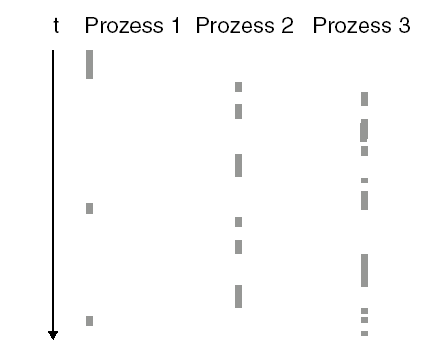
\includegraphics[width=5cm]{images/Concurrency/Quasiparallelitaet.png}
\end{minipage}
\begin{minipage}[c]{10cm}
  \begin{itemize}
    \item Prozesse/Threads warten die meiste Zeit (blocked).
    \item Scheduler ordnet CPU denjenigen Prozessen/Threads zu, die im Zustand ready sind und "'etwas zu tun haben"'
  \end{itemize}
\end{minipage}\\\\
Prozesse/Threads können folgende Zustände und Übergänge erfahren:\\
\begin{minipage}[c]{8cm}
  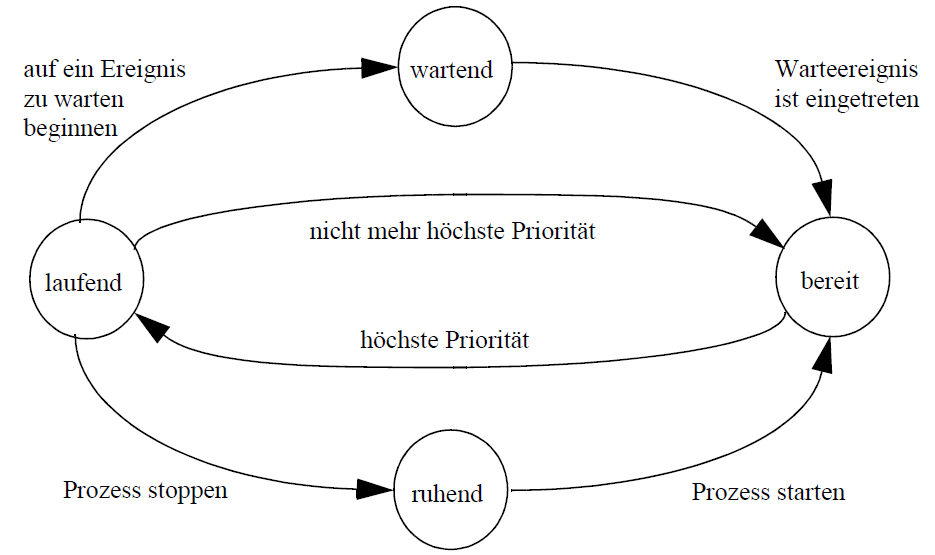
\includegraphics[width=6cm]{images/Concurrency/Prozesszustaende.png}
\end{minipage}
\begin{minipage}[c]{10cm}
  \begin{enumerate}
    \item I/O Operation, Warten auf Bedingung
    \item Scheduler entzieht CPU
    \item Scheduler weist CPU zu
    \item I/O beendet, Bedingung erfüllt
  \end{enumerate}
\end{minipage}

\subsection{Synchonisation: Zugriff auf gemeinsame Ressourcen}
\subsubsection{Kritischer Abschnitt (Critical Section, CS)}
\begin{itemize}
  \item Codebereich, in dem nebenläufige oder parallele Prozesse auf gemeinsame Ressourcen zugreifen. Zu jeder Zeit darf sich höchstens ein Prozess im kritischen Bereich
  befinden.
  \item Der exklusive Zugriff durch höchstens einen Prozess wird mittels gegenseitigem Ausschluss (mutual exclusion, Mutex) sichergestellt.
\end{itemize}

\subsubsection{Lösungsstruktur für gegenseitigen Ausschluss}
\begin{minipage}[c]{2cm}
  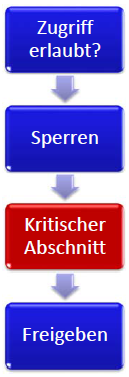
\includegraphics[width=1.5cm]{images/Concurrency/Loesungsstruktur.png}
\end{minipage}
\begin{minipage}[c]{14cm}
  \begin{itemize}
    \item Bei der Zugriffsprüfung wird gewartet, bis der Zugang frei wird \\ \ \\
    \item Beim Sperren wird das Signal auf Rot gesetzt (lock a mutex) \\ \ \\
    \item Beim Freigeben wird das rote Signal wieder gelöscht (unlock a mutex)
  \end{itemize}
\end{minipage}

\subsubsection{Forderungen an die Synchronisation (Dijkstra, 1965)}
\begin{enumerate}
  \item Es dürfen sich nicht zwei Prozesse gleichzeitig in ihrem kritischen Abschnitt befinden (mutual exclusion).
  \item Über die Abarbeitungsgeschwindigkeit, bzw. die Anzahl Prozesse dürfen keine Annahmen getroffen werden.
  \item Kein Prozess darf ausserhalb eines kritischen Abschnitts einen anderen Prozess blockieren.
  \item Jeder Prozess, der am Eingang eines kritischen Abschnitts wartet, muss irgendwann den Abschnitt betreten dürfen (fairness condition).
\end{enumerate}

% \begin{tabbing}
%   \hspace*{1cm}\=\hspace*{4.2cm}\=\hspace*{3cm}\=\hspace*{2.7cm}\= \kill
% \textbf{Synchro-Versuch 1}\\\\
%   \>{\textbf Prozess 1} \> \> \>{\textbf Prozess 2}\\
%   \>\begin{lstlisting}[style=C]
% while(grant != 1)
%     wait();
% CS; //Eintritt in Critical Section
% grant = 2;
%     \end{lstlisting} \> \> \>
%     \begin{lstlisting}[style=C]
% while(grant != 2)
%     wait();
% CS; //Eintritt in Critical Section
% grant = 1;
%     \end{lstlisting} \\\\
%     Forderung 2 nicht erfüllt, da sich alle Prozesse selbst daran hindern 2mal nacheinander daran zu kommen.\\\\
%
% \textbf{Synchro-Versuch 2}\\\\
%    \>{\textbf Prozess 1} \> \> \>{\textbf Prozess 2}\\
%    \>\begin{lstlisting}[style=C]
% while(in2)
%     wait();
% in1 = true;
% CS; //Eintritt in Critical Section
% in1 = false;
%     \end{lstlisting} \> \> \>
%     \begin{lstlisting}[style=C]
% while(in1)
%     wait();
% in2 = true;
% CS; //Eintritt in Critical Section
% in2 = false;
%     \end{lstlisting} \\\\
%     Initialisierung ist nicht gelöst.\\\\
%
% \textbf{Synchro-Versuch 3 (Algorithmus von Peterson)}\\\\
%    \>{\textbf Prozess 1} \> \> \>{\textbf Prozess 2}\\
%    \>\begin{lstlisting}[style=C]
%         request1 = true;
%         grant = 1;
%         while(grant==1 && request2)
%           wait();
%         CS; //Eintritt in Critical Section
%         request1 = false;
%     \end{lstlisting} \> \> \>
%     \begin{lstlisting}[style=C]
%         request2 = true;
%         grant = 2;
%         while(grant==2 && request1)
%           wait();
%         CS;  //Eintritt in Critical Section
%         request2 = false;
%     \end{lstlisting} \\
% \end{tabbing}
% \vspace*{-1cm}

\subsubsection{Synchronisation mit Signalen}
\begin{itemize}
  \item Jeder Prozess wartet vor Betreten des kritischen Bereichs auf ein
  gemeinsames Signal.
  \item Wenn Signal gesetzt $\rightarrow$ kritischer Bereich frei
  \item waitfor(signal) blockiert aufrufenden Prozess, falls signal nicht
  gesetzt
  \item Jeder Prozess, der fertig ist, setzt Signal mit send(signal)
  \item Mehrere Prozesse können gleichzeitig warten
  \item Es ist Aufgabe des Schedulingalgorithmus' bei gesetztem Signal einem der wartenden Prozesse das Betreten des kritischen Abschnitts zu gewähren
\end{itemize}

\begin{tabbing}
  \hspace*{1cm}\=\hspace*{4.2cm}\=\hspace*{3cm}\=\hspace*{2.7cm}\= \kill
  \>{\textbf Prozess 1} \> \> \>{\textbf Prozess 2}\\
  \>\begin{lstlisting}[style=C]
waitFor(signal);
CS;  //Eintritt in Critical Section
send(signal);
    \end{lstlisting} \> \> \>
    \begin{lstlisting}[style=C]
waitFor(signal);
CS;  //Eintritt in Critical Section
send(signal);
    \end{lstlisting} \\\\
 \end{tabbing}
 \vspace*{-1.5cm}

 \subsection{Semaphoren}
 \begin{itemize}
   \item Das Signal für den Zutritt in den kritischen Bereich = Semaphor
   \item Ein Semaphor s hat zwei atomare (= nicht unterbrechbare)
     Operationen
   \begin{itemize}
     \item P(s) : Passieren $\rightarrow$ Beim Eintritt in CS (waitFor)
     \item V(s) : Verlassen $\rightarrow$ Beim Austritt aus CS (send)
   \end{itemize}
   \item Busy waiting
   \begin{itemize}
   \item Beim Busy Waiting warten die Prozesse aktiv in einer Schleife (spin lock)
   \item Wartende Prozesse belasten so unnötigerweise den Prozessor
   \item \textbf{Lösung:} Wartende Prozesse werden in eine Warteschlange eingetragen (sleep und
wakeup)
   \end{itemize}
   \item Probleme der Semaphoren
   \begin{itemize}
    \item Anwendung erfordert viel Disziplin
    \begin{itemize}
      \item Für jedes P(s) braucht es auch ein V(s)
      \item Probleme treten auf, wenn V(s) vergessen geht! (Ressource bleibt besetzt)
    \end{itemize}
    \item In grösseren Programmen können subtile Probleme entstehen, falls z.B. das V(s) in einer if-Bedingung gemacht wird.
    \item Beim Auftreten einer Exception kann das Freigeben ebenfalls schwierig werden.
   \end{itemize}
 \end{itemize}

\subsection{Thread-Synchronisation in C mit POSIX Threads}
\subsubsection{Mutual Exclusion (Mutex)}
\begin{itemize}
  \item A mutex variable acts like a "'lock"' protecting access to a shared data resource
  \item The basic concept of a mutex as used in Pthreads is that only one thread can lock (or own) a mutex variable at any given time. Thus, even if several threads try to lock a mutex, only one thread will be successful.
  \item No other thread can own that mutex until the owning thread unlocks that mutex
  \item Very often the action performed by a thread owning a mutex is the updating of global (shared) variables
  \item This is a safe way to ensure that when several threads update the same variable, the final value is the same as what it would be if only one thread performed the update
  \item The variables being updated belong to a \textbf{critical section}
\end{itemize}
\textbf{A typical mutex sequence:}
\begin{enumerate}
  \item Create and initialize a mutex variable
  \item Several threads attempt to lock the mutex
  \item Only one succeeds and that thread owns the mutex
  \item The owner thread performs some set of actions
  \item The owner unlocks the mutex
  \item Another thread acquires the mutex and repeats the process
  \item Finally the mutex is destroyed
\end{enumerate}

\lstinputlisting[style=C]{snippets/Concurrency/Sync_POSIX.c}

 \subsubsection{Das Monitorprinzip}
 \begin{itemize}
   \item Grundprinzip: Abstrakten Datenyp (ADT) definieren, der genau die Funktionen
   in der Schnittstelle anbietet, die notwendig sind.
   \item Der Aufrufer ruft diese Funktionen auf, er muss sich aber nicht um die
   Synchronisation kümmern.
   \item Die Synchronisation z.B. mit Semaphoren ist in der Implementation des
   Monitors lokal gelöst.
   \item Problem wird einmal im Monitor gelöst, die Aufrufer müssen sich nicht
   mehr darum kümmern.
 \end{itemize}

\subsubsection{Race condition/Starvation/Deadlock}
\begin{description}
 \item[Race Condition]  Das Ergebnis einer Operation hängt von zeitlichen Verhalten bestimmter Einzeloperationen ab.
 \item[Starvation]      Ist ein Zustand, bei dem ein Prozess nie dran kommt (er verhungert). Die Fairness condition besagt, dass Starvation verhindert werden muss.
 \item[Deadlock]        Ist eine Situation in denen sich zwei Prozesse gegenseitig blockieren. Ein Deadlock kann vermieden werden, indem alle Prozesse die gemeinsamen Ressourcen immer in derselben Reihenfolge anfordern.
\end{description}

\subsection{Condition Variables}
\begin{itemize}
  \item Mutexes implement synchronization by controlling thread access to data
  \item \textbf{Condition variables allow threads to synchronize based upon the actual value of data}
  \item Without condition variables, the programmer would need to have threads continually polling (possibly in a critical section), to check if the condition is met
  \item This can be very resource consuming since the thread would be continuously busy in this activity
  \item \textbf{A condition variable is a way to achieve the same goal without polling}
  \item A condition variable is always used in conjunction with a mutex lock
\end{itemize}
\begin{center}
\begin{minipage}{0.8\linewidth}
  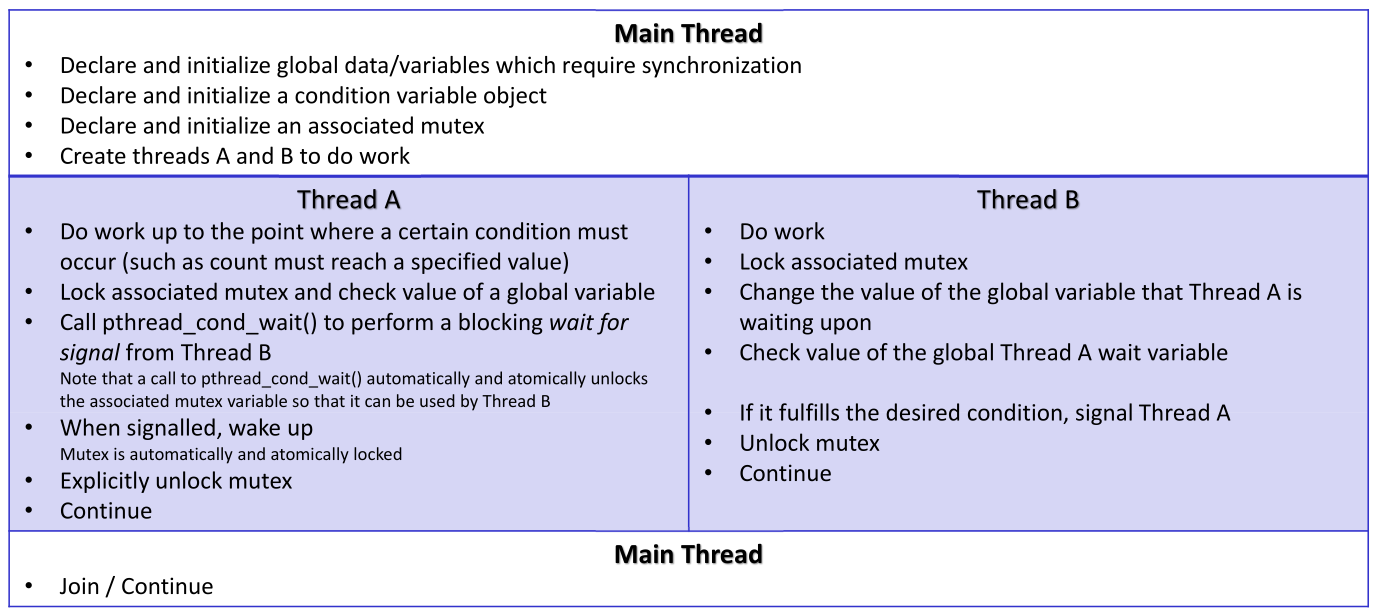
\includegraphics[width=\linewidth]{images/Concurrency/conditionVariablesAblauf}
\end{minipage}
\end{center}

\subsubsection{Creating and destroying condition variables}
\begin{itemize}
  \item Condition variables must be initialized before they can be used\newline
  \lstinline{int pthread_cond_init(pthread_cond_t* condVar, const pthread_condattr_t* attr);}
  \begin{itemize}
    \item condVar: pointer to the condition variable
    \item attr: pointer to a pthread\_condattr\_t structure, often 0 (default attributes)
    \item returns 0 on success
  \end{itemize}
  \item The condition variables shall be destroyed when it's no longer needed\newline
  \lstinline{int pthread_cond_destroy(pthread_cond_t* condVar);}
  \begin{itemize}
    \item condVar: pointer to the condition variable
    \item returns 0 on success
  \end{itemize}
\end{itemize}

\subsubsection{Waiting on condition variables}
\begin{itemize}
  \item waiting on condition variable: blocks calling thread until condition is signalled\newline
  \lstinline{int pthread_cond_wait(pthread_cond_t* condVar, pthread_mutex_t* mutex);}
  \begin{itemize}
    \item condVar: pointer to the condition variable
    \item mutex: pointer to the mutex
    \item returns 0 on success
  \end{itemize}
  \item This routine should be called while mutex is locked
  \item It will automatically release the mutex while it waits
  \item After signal is received and thread is awakened, mutex will be automatically locked for use by the thread
  \item The programmer is then responsible for unlocking mutex when the thread is finished with it
\end{itemize}

\subsubsection{Signaling on condition variables}
\begin{itemize}
  \item Signal on condition variable: unblocks thread blocked on a condition variable\newline
  \lstinline{int pthread_cond_signal(pthread_cond_t* condVar);}
  \begin{itemize}
    \item condVar: pointer to the condition variable
    \item returns 0 on success
  \end{itemize}
  \item This routine is used to signal (or wake up) another thread which is waiting on the condition variable
  \item It should be called after mutex is locked, and must unlock mutex in order for pthread\_cond\_wait() routine to complete
\end{itemize}

\subsubsection{Using condition variables}
\begin{itemize}
  \item This example code demonstrates the use of several Pthread condition variable routines
  \item The main routine creates three threads
  \begin{itemize}
    \item Two of the threads perform work and update a count variable
    \item The third thread waits until the count variable reaches a specific value
  \end{itemize}
  \item The counting thread that reaches the specified count value signals (wakes up) the watching thread waiting on this condition
\end{itemize}

\lstinputlisting[style=C]{snippets/Concurrency/condVariableMain.c}
\lstinputlisting[style=C]{snippets/Concurrency/condVariableIncCount.c}
\lstinputlisting[style=C]{snippets/Concurrency/condVariableWatchCount.c}

\subsubsection{Bounded Buffer Problem}
\begin{itemize}
  \item The problem describes two processes, the producer and the consumer, who share a common, fixed-size buffer used as a queue.
  \item The producer's job is to generate a piece of data, put it into the buffer and start again.
  \item At the same time, the consumer is consuming the data (i.e., removing it from the buffer) one piece at a time.
  \item The problem is to make sure that the producer won't try to add data into the buffer if it's full and that the consumer won't try to remove data from an empty buffer.
  \item The problem can also be generalized to have multiple producers and consumers.
\end{itemize}
\textbf{Solution:}
\begin{itemize}
  \item The solution for the producer is to either go to sleep or discard data if the buffer is full.
  \item The next time the consumer removes an item from the buffer, it notifies the producer, who starts to fill the buffer again.
  \item In the same way, the consumer can go to sleep if it finds the buffer to be empty.
  \item The next time the producer puts data into the buffer, it wakes up the sleeping consumer.
  \item The solution can be reached by means of inter-process/thread communication, typically using semaphores (mutexes).
  \item An inadequate solution could result in a deadlock where both processes are waiting to be awakened.
\end{itemize}

\subsection{POSIX Interprocess Communication (IPC)}
\begin{itemize}
  \item POSIX provides the following IPC mechanisms in the POSIX:XSI extension:
  \begin{itemize}
    \item Message queues in sys/msg.h
    \item Semaphores in sys/sem.h
    \item Shared Memory in sys/shm.h
  \end{itemize}
  \item These mechanisms allow unrelated processes to exchange information in a reasonably efficient way
\end{itemize}

\subsection{RAII (Resource Acquisition Is Initialisation)}
\subsubsection{Motivation}
\begin{itemize}
  \item Ressourcen (z.B. Datei, Speicher, etc.) müssen vor dem Gebrauch grundsätzlich angefordert werden
  \item Nach Abschluss des Gebrauchs einer Ressource muss diese wieder freigegeben werden
  \item Die saubere Anforderung und Freigabe ist fehlerträchtig
  \item RAII löst diese Aufgabe elegant und zuverlässig
\end{itemize}

\subsubsection{Idee hinter RAII}
\begin{itemize}
  \item Die Anforderung und Freigabe einer Ressource wird mit Hilfe einer Klasse implementiert:
  \begin{itemize}
    \item der Konstruktor fordert die Ressource an
    \item der Destruktor gibt sie wieder frei
  \end{itemize}
  \item Die verwendete Ressource kann wie ein Objekt behandelt werden. Sobald das Objekt seine Gültigkeit verliert (z.B. out-of-scope), wird durch den Destruktor die Ressource "'automatisch"' freigegeben.
\end{itemize}

\subsubsection{Anwendung bei Heapobjekten}
\begin{itemize}
  \item Wie kann man sicher gehen, dass ein Objekt, welches auf dem Heap angelegt wurde, auch wieder mittels delete sicher gelöscht wird?
  \begin{itemize}
    \item Exceptions können dazwischen kommen
    \item C++03 kennt kein finally bei Exception-Handling
  \end{itemize}
\end{itemize}
\begin{lstlisting}[style=C,escapechar=!]
void f()
{
  Person* p = new Person("irgendwer");
  // mach etwas mit p!\tikz[remember picture] \node [] (a) {};!
  delete p;
}
\end{lstlisting}
\begin{tikzpicture}[remember picture, overlay,
  every edge/.append style = { ->, thick, >=stealth, dashed, line width = 1pt},
  every node/.append style = { align = left, minimum height = 10pt, font = \bfseries, fill= green!20},
  text width = 7.5cm]
  \node [right=5cm of a] (A) {was ist, wenn hier eine Exception geworfen wird?};
  \draw (A.west) edge (a.east);
\end{tikzpicture}
\textbf{Lösung:}
\begin{itemize}
  \item Kapsle die dynamisch erzeugte Ressource mit einem Handle-Objekt auf dem Stack
  \begin{itemize}
    \item Ideal std::shared\_ptr\textless T\textgreater aus Header \textless memory\textgreater
  \end{itemize}
  \item Der Destruktor dieses Handle-Objekts räumt beim Verlassen des Scop automatisch auf. Das gilt auch für externe Ressourcen wie Files
\end{itemize}
\begin{lstlisting}[style=C,escapechar=!]
#include <memory>
void f()
{
  std::shared_ptr<Person> p(new Person("irgendwer"));
  // mach etwas mit p
}!\tikz[remember picture] \node [] (a) {};!
\end{lstlisting}
\begin{tikzpicture}[remember picture, overlay,
  every edge/.append style = { ->, thick, >=stealth, dashed, line width = 1pt},
  every node/.append style = { align = left, minimum height = 10pt, font = \bfseries, fill= green!20},
  text width = 11cm]
  \node [right=5cm of a] (A) {Beim Verlassen des Blocks räumt der Destruktor von shared\_ptr automatisch auf und löscht die Person};
  \draw (A.west) edge (a.east);
\end{tikzpicture}

\subsubsection{Anwendung bei Mutex}
\begin{itemize}
  \item Wie kann man sicher gehen, dass eine Mutex, die mit lock(m) angefordert wurde, in jedem Fall auch wieder mit unlock(m) freigegeben wurde?
  \begin{itemize}
    \item Exceptions könne dazwischen kommen
    \item Freigabe auch bei vorzeitigem Ausstieg mit return
  \end{itemize}
\end{itemize}
\begin{lstlisting}[style=C,escapechar=!]
static pthread_mutex_t m;
// ...
void f()
{
  pthread_mutex_lock(&m);
  // mach etwas in kritischem Abschnitt!\tikz[remember picture] \node [] (a) {};!
  pthread_mutex_unlock(&m);   // auf keinen Fall vergessen
}
\end{lstlisting}
\begin{tikzpicture}[remember picture, overlay,
  every edge/.append style = { ->, thick, >=stealth, dashed, line width = 1pt},
  every node/.append style = { align = left, minimum height = 10pt, font = \bfseries, fill= green!20},
  text width = 6.5cm]
  \node [right=4cm of a] (A) {was ist, wenn hier eine Exception geworfen wird?};
  \draw (A.west) edge (a.east);
\end{tikzpicture}
\textbf{Lösung:}\\
Kritischer Abschnitt muss in einen Block gepackt werden.
\begin{lstlisting}[style=C,escapechar=!]
class ResourceLock
{
  public:
    ResourceLock(pthread_mutex_t& mx) : mutex(mx) { pthread_mutex_lock(&mutex); }
    ~ResourceLock() { pthread_mutex_unlock(&mutex); }
  private:
    pthread_mutex_t& mutex; // ref to mutex of shared resource
};

void f()
{
  //...
  {
    ResourceLock lock(myMutex);
    // mach etwas in kritischem Abschnitt
  }!\tikz[remember picture] \node [] (b) {};!
}
\end{lstlisting}
\begin{tikzpicture}[remember picture, overlay,
  every edge/.append style = { ->, thick, >=stealth, dashed, line width = 1pt},
  every node/.append style = { align = left, minimum height = 10pt, font = \bfseries, fill= green!20},
  text width = 7.5cm]
  \node [right=8cm of b] (B) {Hier wird lock automatisch freigegeben, egal ob der Block ordentlich oder wegen einer Exception verlassen wird.};
  \draw (B.west) edge (b.east);
\end{tikzpicture}



\subsection{Petri-Netze}
\subsubsection{Was sind Petri-Netze?}
\begin{itemize}
\item Petri-Netze (Petri Nets) sind eine graphische Darstellung von parallelen Prozessen.
\item Petri-Netze sind bipartite Graphen (Graphen mit zwei Arten von Knoten)
\item Petri-Netze sind mathematische Modelle. Es bestehen Methoden zur
Optimierung und formalen Verifikation (Deadlock-Analyse).
\end{itemize}
\subsubsection{Elemente}
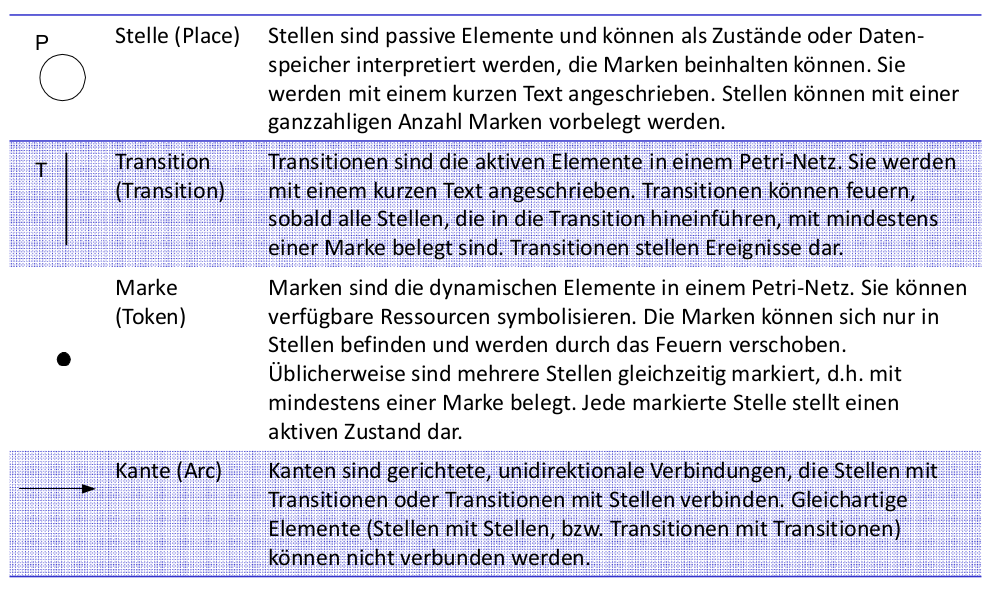
\includegraphics[width=15cm]{images/Concurrency/PetriNetzeElemente}
\newpage
\subsubsection{Feuern von Transitionen}
\begin{itemize}
\item Das Feuern ist die einzige Aktion, die in einem Petri-Netz ausgeführt werden kann.
\item Eine Transition kann dann und nur dann feuern, wenn alle Stellen, die in die Transition hineinführen (Eingabestellen), mit mindestens einer Marke belegt sind. Dann wird bei jeder dieser Stellen eine Marke abgezogen.
\item Jede Stelle, die aus
dieser Transition hinausführt (Ausgabestellen), erhält umgekehrt eine Marke.
\item Das Feuern ist somit das Verschieben von Marken unter definierten Bedingungen.
\end{itemize}
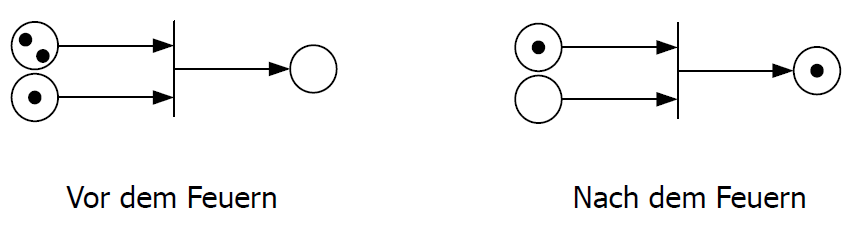
\includegraphics[width=8cm]{images/Concurrency/Petri1}

\subsubsection{Grundstrukturen}
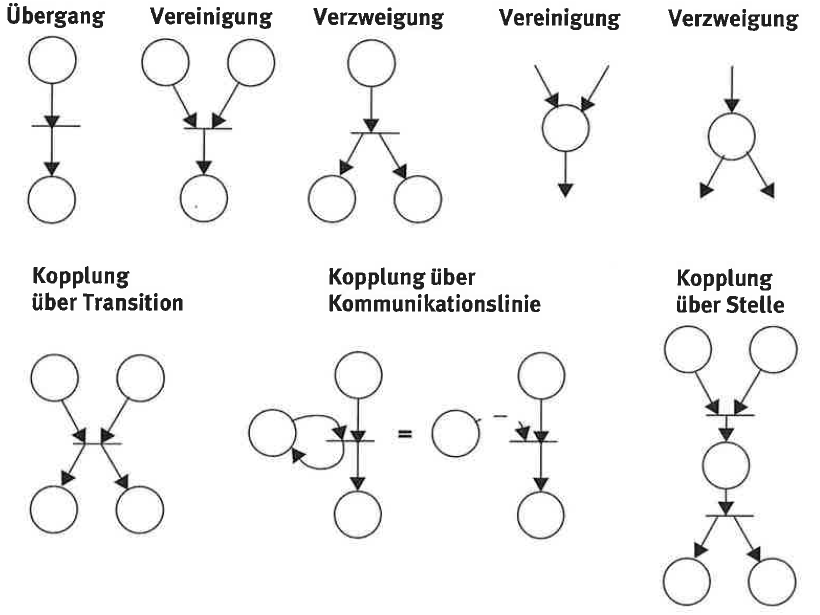
\includegraphics[width=9cm]{images/Concurrency/Petri2}

\vspace*{-1cm}
\subsubsection{Beispiel}
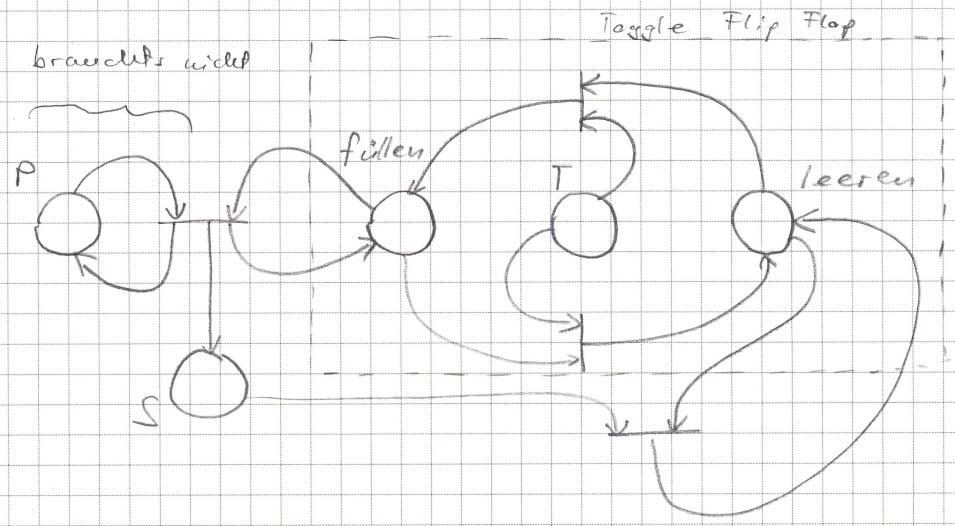
\includegraphics[width=10cm]{images/Concurrency/Petri3}\\
In diesem Beispiel produziert der Produzent P bei jedem Takt ein Marke in S. Sobald eine Marke in T gesetzt wird, wird S geleert. P ist während dieses Vorgangs gesperrt. P produziert wieder, wenn erneut eine Marke in T gesetzt wird. Der Leerprozess wird dann gestoppt.
